\title{Milestone 4}
\author{Singularity Software}
\date{\today}

\documentclass[12pt]{article}
\usepackage[a4paper]{geometry}
\usepackage{makeidx}
\usepackage{lscape}
\usepackage{amsmath}
\usepackage{graphicx}
\usepackage[final]{pdfpages}

\geometry{top=1.0in, bottom=1.0in, left=1.0in, right=1.0in} % Sets the margins

\setlength{\parindent}{0pt} % Fixes the paragraph spacing problem

\renewcommand*\arraystretch{1.5}

\begin{document}

\begin{center}
	\LARGE{Milestone 4} \\
	\Large{\textit{Singularity Software}} \\
	\vspace{.05in}
	\normalsize{\today} \\
\end{center}

\section*{A Non-Trivial Technical Change}
With images functioning correctly in the emulator, the next element that needed to be incorporated into the functioning system was the concept of a sound. For the purposes of an application or game, sounds prove to be a useful mechanism of indicating success and/or failure or setting the mood with a little background music. \\\\
In the Sifteo level – at least, what we decided still needed to be our own implementation – there are two entities that deal with sounds: Sound and SoundSet. The former is representative of one sound object, and the latter is an aggregation of all of the available sounds for the application running in the emulator. \\\\
Much like with loading images, when an application is loaded, all of its available sound assets are loaded as well (located in that application’s assets/sounds directory). Then, from within the application, a sound can be created and played using intuitive methods Play, Pause, Resume, and Stop (along with other bits of functionality like setting the volume level). The interface is obvious, but the implementation to funnel these method calls up to our application and view layers is not so immediately obvious. \\\\
The primary technical issue comes with utilizing the capabilities of Silverlight to do what we need without overstepping our needs. Images did not present such an issue because for the purposes of the emulator, an image is drawn to the screen and then is lost to the user forever. However, sounds have a state and can be changed after being “drawn” to the window. This presents a problem, because our current design does not facilitate communication from the domain (Sifteo) layer to the UI layer, as shown in the following partial class diagram:
\begin{center}
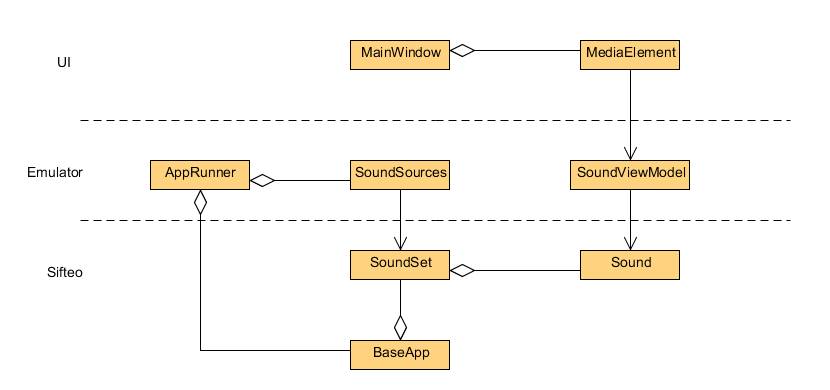
\includegraphics[scale=.5]{classDiagram.png}
\end{center}
For the purposes of our emulator, we have a MainWindow view which encompasses the emulator as a whole, but all we need to analyze this issue is to realize that within that MainWindow there is an ItemsControl bound to the collection of SoundViewModels in MainWindowViewModel. Each SoundViewModel is the data context of a MediaElement, Silverlight’s readily-available entity for playing sounds (and videos too!). \\\\
However, note the issue of direction of flow, which is in some ways slightly opposite of what may be expected in a typical MVVM application. The MediaElement is bound to a SoundViewModel, which has access to a Sound object. We know from implementing the imaging functionality that we can effectively communicate back-and-forth between the viewmodels and Sifteo-level objects, so that is not an issue. But how do we link up the following communications without breaking the rules of MVVM?
\begin{center}
\begin{tabular}{c | c}
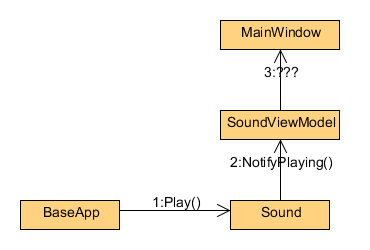
\includegraphics[scale=.45]{basicCommunication.png}	&
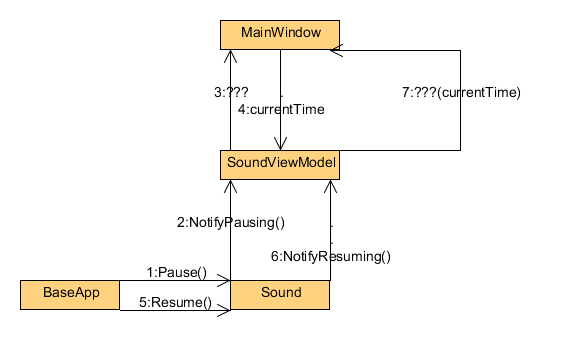
\includegraphics[scale=.45]{pauseAndResume.png} \\
(Basic playing communication) &
(Pause and resume communication)
\end{tabular}
\end{center}
The solution we decided upon was to maintain separate collections. When a sound is created/paused/stopped, it is placed in the InactiveSounds collection. When it is played or resumed, it is subsequently added to the ActiveSounds collection, and this is what the MediaElements are bound to. This allows us to successfully keep track of which sounds we know about and can use without having to break the rules and make calls to the MediaElement’s interface. \\\\
Now we have solved the issue of being able to keep the emulator in the loop about which sounds should be playing, but one more incident arises. When we pause a sound, we need to have the ability to resume the sound at the same point in its track sometime in the future. This is easy enough with a straight-up Silverlight implementation because the MediaElement has Pause and Resume methods built in. However, because we want to avoid that unnecessary dependency on the MediaElement by the SoundViewModel, we have to take a slightly more complicated approach to maintain a sound’s playback position. \\\\
The naive solution is to just add a property to the SoundViewModel which is the direct binding of the MediaElement’s Position attribute. And this is on the right track, but unfortunately it won’t quite work. The viewmodel will always get the right data, and when Pause is called the viewmodel knows the point at which it needs to resume. However, when Resume is called, there is no intuitive way to let the “view” know where it needs to start. The viewmodel does not directly know about the MediaElement, and the MediaElement will update its own position to be the beginning of the track before even considering the viewmodel’s opinion of where it should begin. \\\\
To solve this one last problem, we need only exploit one more built-in feature of the MediaElement as well as the libraries available to us. When the MediaElement is initialized, its natural instinct is to set its starting position to be the beginning of the sound. Instead, we indicate to the MediaElement that we want to take control as soon as it is loaded. By converting the MediaOpened event to a command we can call on the data context (in our case the viewmodel), we take control without giving any notion to the viewmodel of the entity which it is serving. The XAML code ends up quite simply looking like \\\\
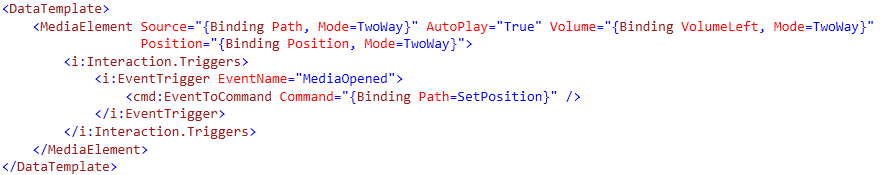
\includegraphics[scale=.65]{xamlCode.png} \\\\
and we add a short command call to the SoundViewModel to force-update the sound’s position to the value before pausing (which will propagate to the MediaElement via the binding): \\\\
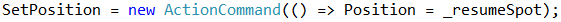
\includegraphics[scale=.65]{commandCode.png} \\\\
Though it took some time to traverse the options, the final design solves the problem while also maintaining the proper MVVM structure we sought out in the beginning. If in the future we decide to implement the UI portion of the emulator in a different way, we would have very little trouble porting out our Sifteo and application layers to use alongside a different framework. Lower coupling is maintained between layers while entities strongly preserve their individual responsibilities with respect to domain level calls and interface level updates.

\section*{Sprints 3 \& 4 Backlogs}
The following pages show the backlog for the previous sprint (sprint 3) and the new sprint (sprint 4). The one unfinished task from the previous sprint has been moved to the new sprint.\\

The previous sprint's completed tasks list is larger than usual because of our decompilation and subsequent Silverlight recompilation of parts of Sifteo.dll. Any task referencing a Sifteo.MathExt or Sifteo.Util class (e.g. StateMachine) falls under this category.\\

We are opting not to do TDD for the new sprint.\\

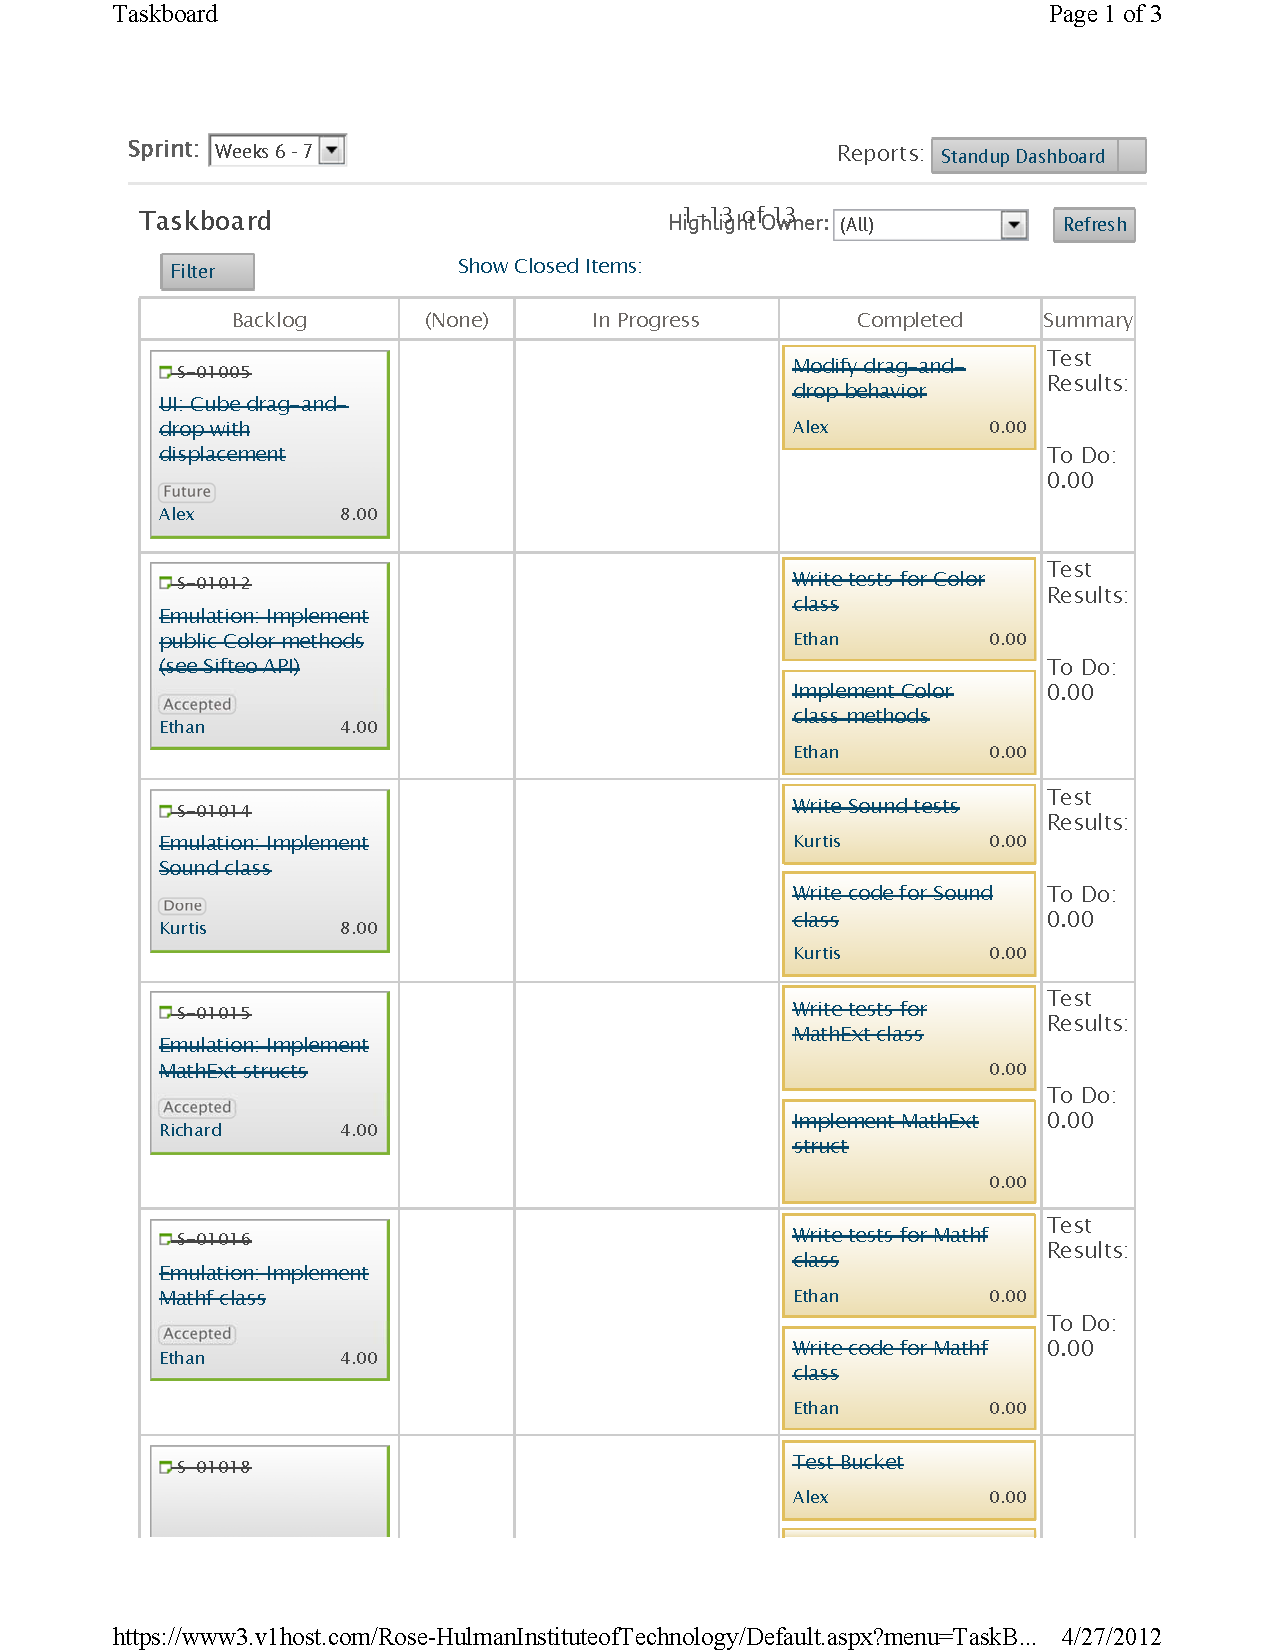
\includepdf[pages={1-3}]{pdfs/MS4VersionOne/OldSprintDetail.pdf}

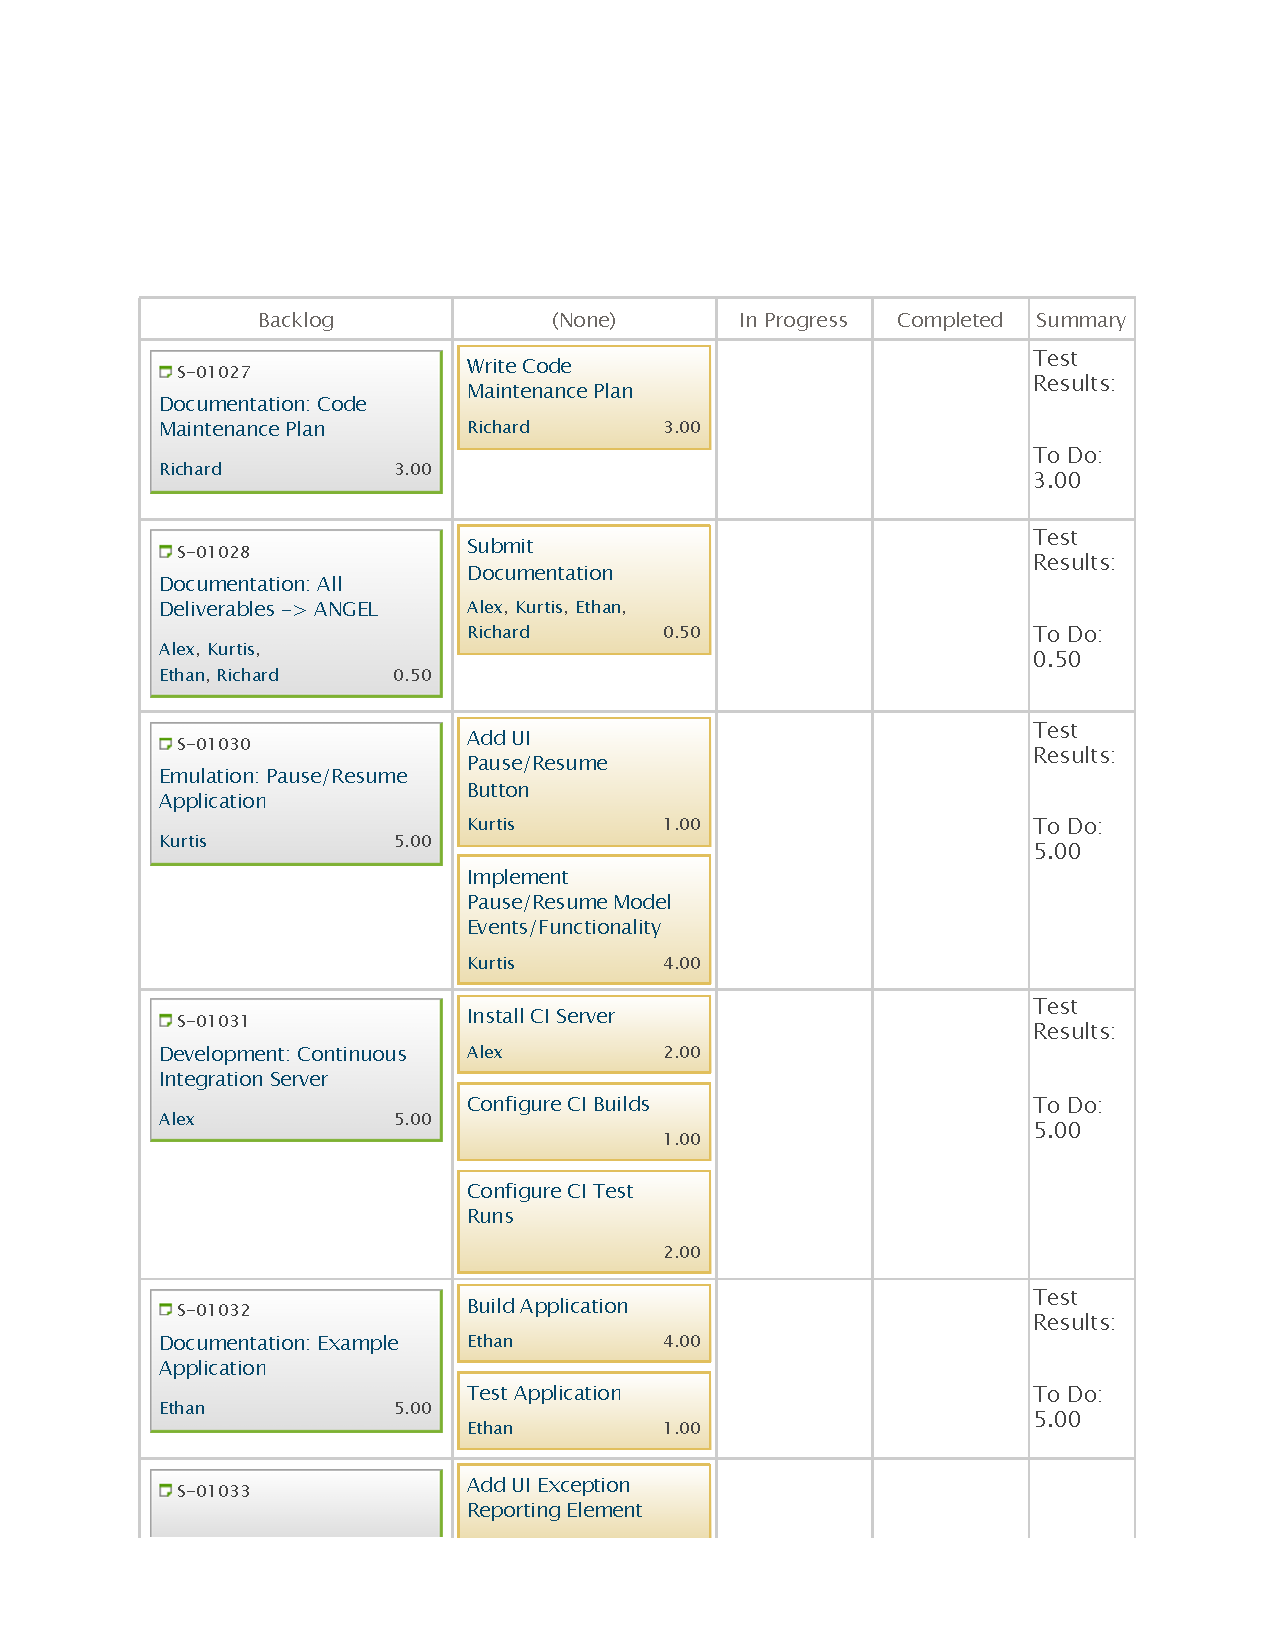
\includepdf[pages={1-2}]{pdfs/MS4VersionOne/NewSprintDetail.pdf}

\clearpage
        
\end{document}
